\documentclass[11pt]{article}
\usepackage{amsmath}
\usepackage{amssymb}
\usepackage{geometry}
\usepackage{graphicx}
\usepackage{algorithm}
%\usepackage{algorithmic}
\usepackage{algpseudocode}
\geometry{margin=0.7in}
\setlength\parindent{0pt}
\setlength{\parskip}{3pt}

\begin{document}
\textbf{2D Sonar Simulator: } Camille Wardlaw, Manuel Valencia, Demircan Tas 


\textbf{(a) Internal Team Meeting and PM Plan}\\
\textbf{Team Meeting:} Monday September 22, 9--11am (all team members present)

\textbf{Graded Project Milestones:}
PM1: required for all. PM2 or PM3: linear sparse system solvers. PM5: required since the problem involves time simulation. PM6: possible, for model order reduction of large grids. We will not have PM4 graded because our problem is fully linear.

\textbf{(b) System Description}

\begin{figure}[h]
    \centering
    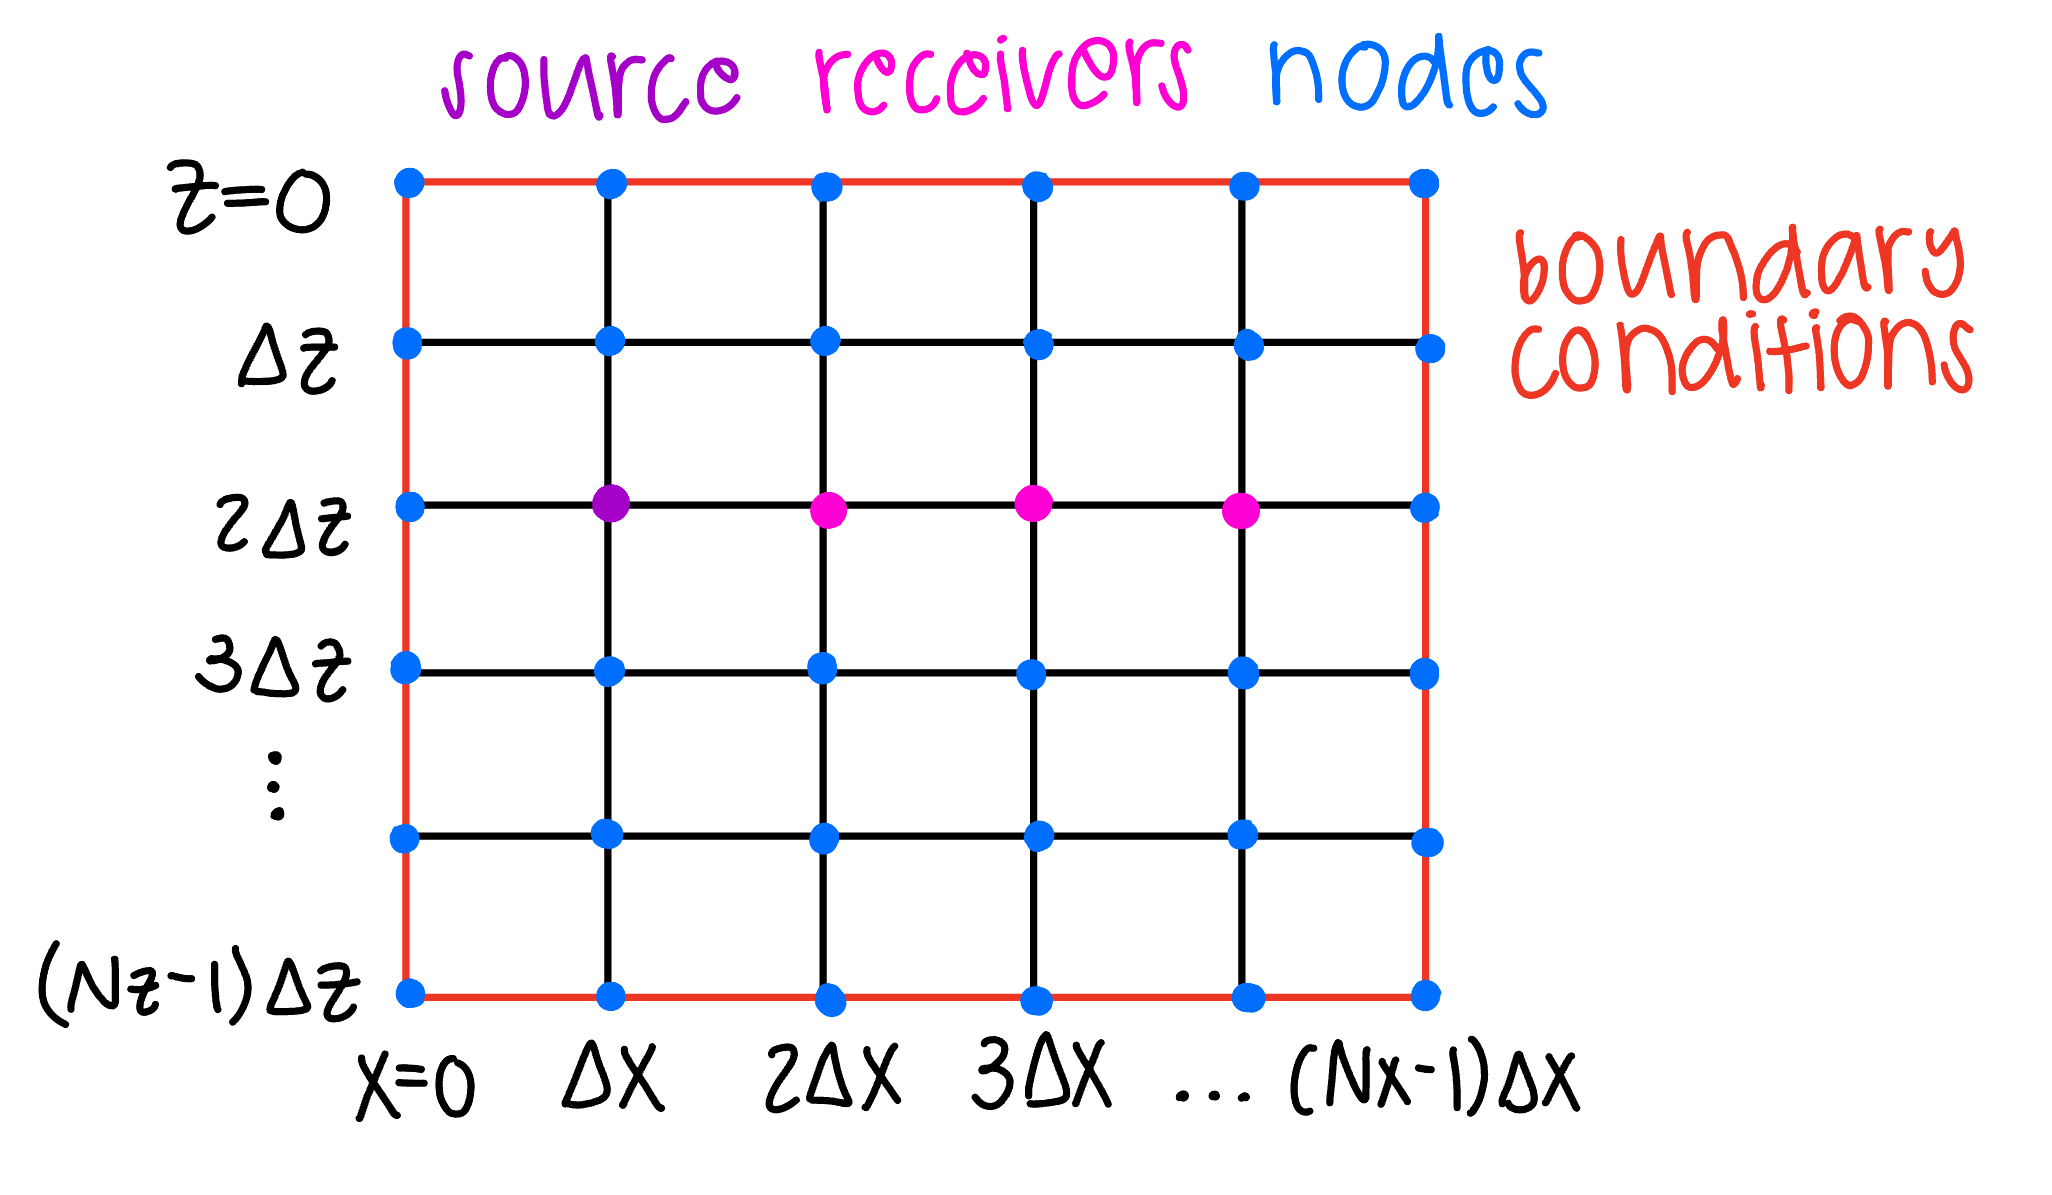
\includegraphics[width=0.5\linewidth]{system.jpeg}
    \caption{2D Cartesian grid in $(x,z)$ space.}
\end{figure}

The sonar simulator models wave propagation on a uniform rectangular grid in $(x,z)$ space. Each grid point $(i,j)$ represents a small control volume of fluid.

\textbf{Formulation Type:} Nodal formulation with nodes representing grid points $(i,j)$ with $i \in [0,N_x-1]$ and $j \in [0,N_z-1]$.

\textbf{Nodal Quantities:} Acoustic pressure $p_{i,j}$ [Pa], and time derivative of pressure $w=\partial p_{i,j}/\partial t$ [Pa/s]


\textbf{Nodal Equation:} We use the scalar acoustic wave equation with linear damping:
\[
\frac{\partial^2 p}{\partial t^2} + \alpha \frac{\partial p}{\partial t} = c^2 \nabla^2 p + s(x,z,t)
\]

where $p(x,z,t)$ is acoustic pressure [Pa], $c$ is sound speed [m/s], $\alpha$ is a bulk absorption coefficient [1/s], and $s$ is a source term.

\textbf{First-Order Formulation:} Introduce $w=\partial p/\partial t$. The PDE becomes a first-order system:
\[
\frac{d}{dt}
\begin{bmatrix}p \\ w\end{bmatrix}
=
\underbrace{\begin{bmatrix}
0 & I \\ c^2 \nabla^2 & -\alpha I
\end{bmatrix}}_{A}
\begin{bmatrix}p \\ w\end{bmatrix}
+
\underbrace{\begin{bmatrix} 0 \\ s \end{bmatrix}}_{B u(t)}
\]

This yields a linear time-invariant ODE system $
\dot{\mathbf{x}} = A\mathbf{x} + B u$ with state vector $\mathbf{x} = [p; w] \in \mathbb{R}^{2N}$. Here $s(x,z,t) = b(x,z)\,u(t)$ is factored into a spatial vector $b$ and temporal input $u(t)$.

\textbf{Spatial Discretization} The Laplacian $\nabla^2 p$ is approximated by a 5-point finite-difference stencil:
\[
(\nabla^2 p)_{i,j} \approx
\frac{p_{i+1,j}-2p_{i,j}+p_{i-1,j}}{\Delta x^2} +
\frac{p_{i,j+1}-2p_{i,j}+p_{i,j-1}}{\Delta z^2}
\]

Boundary rows in the discrete Laplacian $L$ are modified for:
\begin{itemize}
    \item Top boundary: pressure-release ($p=0$)
    \item Bottom: rigid wall ($\partial p/\partial z=0$)
    \item Left/right: simple absorbing (one-sided stencil approximation)
\end{itemize}

\textbf{State-Space Matrices} With $N=N_x N_z$ grid nodes:
\[
A = 
\begin{bmatrix}
0_{N\times N} & I_{N} \\
L & -\alpha I_{N}
\end{bmatrix},
\qquad
B = \begin{bmatrix} 0 \\ b \end{bmatrix}
\]

where $L \in \mathbb{R}^{N\times N}$ is the discrete Laplacian scaled by $c^2$.  \\
\textit{Note:} The left/right boundary condition is a simple one-sided stencil to reduce reflections; it is not a full PML or impedance-matched boundary.
The source vector $b$ has a single nonzero entry at the sonar location $(i_\mathrm{src},j_\mathrm{src})$:
\[
b_{k_\mathrm{src}} = \frac{1}{\Delta x \Delta z}
\]
\textbf{Components and Component Quantities:} Components represent the acoustic propagation paths between nodes. However, on the nodal formulation, there are no explicit branch variables. Neighbor-to-neighbor coupling is carried by the Laplacian operator $\nabla^2$, which plays the role of implicit components connecting adjacent nodes.

\textbf{Parameters:}
$\mathbf{p} = \{c, \alpha, N_x, N_z, L_x, L_z, i_\mathrm{src}, j_\mathrm{src}, \text{hydrophones}\}\
$

\textbf{Hydrophone array (implementation):}
\[\text{hydrophones} = \{ z\_\mathrm{pos},\; x\_\mathrm{indices},\; n\_\mathrm{phones} \} \]
We denote the source index as $(i_\mathrm{src}, j_\mathrm{src})$ in the derivation; in code these correspond to `p['sonar_ix']`, `p['sonar_iz']`.

\textbf{Input:} Gaussian-windowed pulse, source excitation.
\[
u(t) = A_0 \sin(2\pi f_0 t) \exp\!\left[-\frac{(t-t_0)^2}{\sigma^2}\right]
\]

\textbf{Outputs:} Received pressure at hydrophone locations $(i_{\mathrm{rx},h},j_{\mathrm{rx},h}), \; h=1,\dots,H$:

\[
\mathbf{y}(t) = 
\begin{bmatrix}
p_{k_{\mathrm{rx},1}}(t) \\
p_{k_{\mathrm{rx},2}}(t) \\
\vdots \\
p_{k_{\mathrm{rx},H}}(t)
\end{bmatrix}
\in \mathbb{R}^{H}
\]

or equivalently, in compact state-space form: $\mathbf{y}(t) = C \mathbf{x}(t)$, where $C \in \mathbb{R}^{H \times 2N}$ is a selector matrix that picks the pressure components of the state vector at the chosen hydrophone indices.

\textbf{Units and Normalization:}
\begin{itemize}
    \item $p$ in Pascals [Pa], $w=\dot p$ in [Pa/s], $c$ in [m/s], $\alpha$ in [1/s].
    \item $L$ embeds the spatial scaling $c^2/\Delta x^2$ and $c^2/\Delta z^2$.
    \item The source enters $\dot w = c^2 L p - \alpha w + b\,u(t)$, with $b_{k_\mathrm{src}} = 1/(\Delta x\,\Delta z)$. With this choice, $u(t)$ must have units [Pa\,$\cdot$\,m$^2$/s$^2$] so that $b\,u(t)$ has units [Pa/s$^2$]. In practice we use a normalized $u(t)$ for demonstration; amplitudes are chosen for numerical clarity rather than physical calibration.
\end{itemize}

\newpage

\begin{algorithm}[h]
\caption{Function \texttt{evalf(x,p,u)}}
\begin{algorithmic}[1]
\State \textbf{Input:} state $\mathbf{x} = [p;w]$, parameters $\mathbf{p}$, input $u(t)$
\State \textbf{Output:} right-hand side $\dot{\mathbf{x}} = f(\mathbf{x},\mathbf{p},u)$
\vspace{6pt}
\State Partition $\mathbf{x}$ into nodal fields:
\[
p \in \mathbb{R}^N, \quad w \in \mathbb{R}^N
\]
\State Initialize $f_p, f_w \in \mathbb{R}^N$
\State Enforce nodal equations:
\begin{align*}
f_p &= w \qquad \;\; \text{(definition of $w=\dot p$)} \\
f_w &= c^2 L p - \alpha w + b\,u(t)
\end{align*}
where $L$ is the discrete Laplacian matrix and $b$ the source vector
\State Apply boundary conditions by modifying rows of $L$ and $b$ as needed
\State Assemble output:
\[
f(\mathbf{x},\mathbf{p},u) =
\begin{bmatrix}
f_p \\ f_w
\end{bmatrix}
\]
\end{algorithmic}
\end{algorithm}

\begin{algorithm}[h]
\caption{Function \texttt{jacobian(x, p, u)} — ODE form (BCs enforced outside $f$)}
\begin{algorithmic}[1]
\State \textbf{State:} $\mathbf{x}=\begin{bmatrix}p\\ w\end{bmatrix}\in\mathbb{R}^{2N}$ \quad
\textbf{Dynamics:}\quad
$\dot p = w,\quad \dot w = c^2 L p - \alpha w + b\,u(t)$
\State \textbf{Return:} $J=\dfrac{\partial f}{\partial x}\in\mathbb{R}^{2N\times 2N}$
\vspace{4pt}
\State Precompute / have available: sparse $L\in\mathbb{R}^{N\times N}$, identity $I_N$
\State Assemble block Jacobian (time-invariant here):
\[
J \;=\;
\begin{bmatrix}
\frac{\partial \dot p}{\partial p} & \frac{\partial \dot p}{\partial w}\\[2pt]
\frac{\partial \dot w}{\partial p} & \frac{\partial \dot w}{\partial w}
\end{bmatrix}
\;=\;
\begin{bmatrix}
0 & I_N\\[2pt]
c^2 L & -\alpha I_N
\end{bmatrix}.
\]
\State \textbf{Note:} input $u(t)$ does not appear in $J$ (it is additive via $b\,u(t)$).
\State \textbf{Return} $J$
\end{algorithmic}
\end{algorithm}

\end{document}
